\documentclass[xetex,mathserif,serif]{beamer}
\usepackage{polyglossia}
\setdefaultlanguage[babelshorthands=true]{russian}
\usepackage{minted}

\useoutertheme{infolines}

\setmainfont{FreeSans}
\newfontfamily{\russianfonttt}{FreeSans}

\title{Хорошие практики ООП}
\author[Юрий Литвинов]{Юрий Литвинов \newline \textcolor{gray}{\small\texttt{yurii.litvinov@gmail.com}}}
\date{12.07.2017г}

\begin{document}
	
	\frame{\titlepage}

	\section{Декомпозиция и модульность}

	\begin{frame}
		\frametitle{Модульность}
		\begin{itemize}
			\item Разделение системы на компоненты
			\item Потенциально позволяет создавать сколь угодно сложные системы
		\end{itemize}
		\vskip 1cm
		\begin{center}
			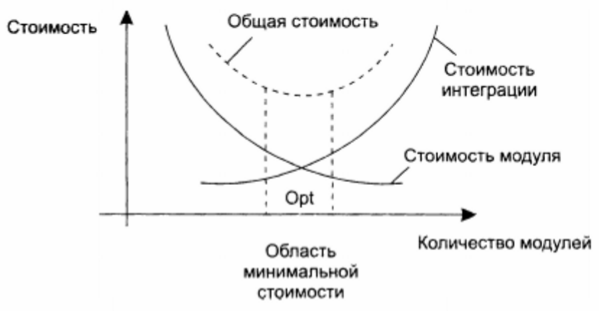
\includegraphics[width=0.5\textwidth]{modulesCost.png}
		\end{center}
	\end{frame}

	\begin{frame}
		\frametitle{Информационная закрытость}
		\begin{itemize}
			\item Со­держание модулей должно быть скрыто друг от друга
			\begin{itemize}
				\item Все модули независимы
				\item Обмениваются только информацией, необходимой для работы
				\item Доступ к операциям и структурам данных модуля ограничен
			\end{itemize}
			\item Обеспечивается возможность разработки модулей различными независимыми коллективами
			\item Обеспечивается лёгкая модификация системы
		\end{itemize}
	\end{frame}

	\begin{frame}
		\frametitle{Подходы к декомпозиции}
		\begin{itemize}
			\item Восходящее проектирование
			\item Нисходящее проектирование
			\begin{itemize}
				\item Постепенная реализация модулей
				\item Строгое задание интерфейсов
				\item Активное использование ``заглушек''
				\item Модули
				\begin{itemize}
					\item Четкая декомпозиция
					\item Минимизация
					\item Один модуль --- одна функциональность
					\item Отсутствие побочных эффектов
					\item Независимость от других модулей
					\item Принцип сокрытия данных
				\end{itemize}
			\end{itemize}
		\end{itemize}
	\end{frame}

	\begin{frame}
		\frametitle{Объекты}
		\begin{itemize}
			\item Objects may contain data, in the form of fields, often known as attributes; and code, in the form of procedures, often known as methods --- \textbf{\href{https://en.wikipedia.org/wiki/Object-oriented\_programming}{Wikipedia}}
			\item An object stores its state in fields and exposes its behavior through methods --- \textbf{\href{https://docs.oracle.com/javase/tutorial/java/concepts/object.html}{Oracle}}
			\item Each object looks quite a bit like a little computer --- it has a state, and it has operations that you can ask it to perform --- \textbf{\href{http://amzn.to/1PBmQpm}{Thinking in Java}}
			\item An object is some memory that holds a value of some type --- \textbf{\href{http://amzn.to/1XyGCtk}{The C++ Programming Language}}
			\item An object is the equivalent of the quanta from which the universe is constructed --- \textbf{\href{http://amzn.to/266oJr4}{Object Thinking}}
		\end{itemize}
	\end{frame}

	\section{Некоторые принципы ОО-проектирования}

	\begin{frame}
		\frametitle{Определение объектов реального мира}
		\begin{itemize}
			\item Определение объектов и их атрибутов
			\item Определение действий, которые могут быть выполнены над каждым объектом
			\item Определение связей между объектами
			\item Определение интерфейса каждого объекта
		\end{itemize}
		\begin{center}
			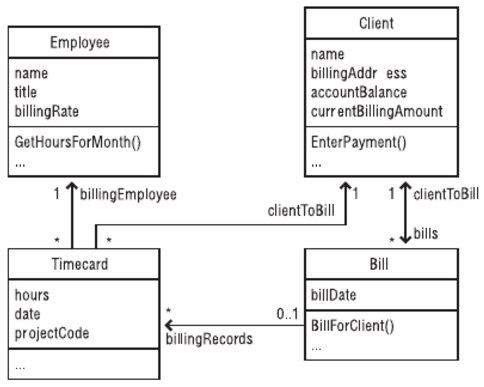
\includegraphics[width=0.4\textwidth]{billDomainModel.png}
		\end{center}
	\end{frame}

	\begin{frame}
		\frametitle{Согласованные абстракции}
		\begin{itemize}
			\item Выделение существенных характеристик объекта и игнорирование несущественных
			\item Определение его концептуальных границы с точки зрения наблюдателя
			\begin{itemize}
				\item Определение интерфейсов
			\end{itemize}
			\item Управление сложностью через фиксацию внешнего поведения
			\item Необходимы разные уровни абстракции
		\end{itemize}
		\begin{center}
			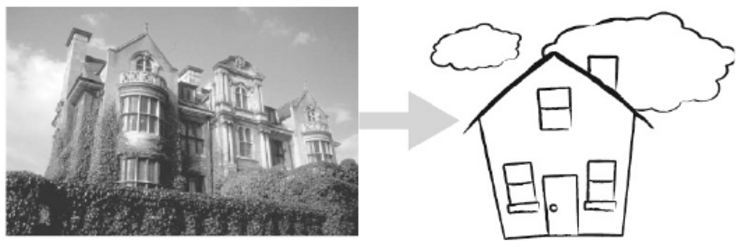
\includegraphics[width=0.55\textwidth]{abstraction.png}
		\end{center}
	\end{frame}

	\begin{frame}
		\frametitle{Инкапсуляция деталей реализации}
		\begin{itemize}
			\item Отделение друг от друга внутреннего устройства и внешнего поведения
			\item Изолирование контрактов интерфейса от реализации
			\item Управление сложностью через сокрытие деталей реализации
		\end{itemize}
		\vskip 1.5cm
		\begin{center}
			
\includegraphics[width=0.55\textwidth]{incapsulation.png}
		\end{center}
	\end{frame}

	\begin{frame}
		\frametitle{Сокрытие ``лишней'' информации}
		\begin{columns}
			\begin{column}{0.65\textwidth}
				\begin{itemize}
					\item Изоляция ``личной'' информации
					\begin{itemize}
						\item секреты, которые скрывают сложность
						\item секреты, которые скрывают источники изменений
					\end{itemize}
					\item Барьеры, препятствующие сокрытию
					\begin{itemize}
						\item избыточное распространение информации
						\item поля класса как глобальные данные
						\item снижение производительности
					\end{itemize}
				\end{itemize}
			\end{column}
			\begin{column}{0.3\textwidth}
				\vskip 3cm
				\begin{flushright}
					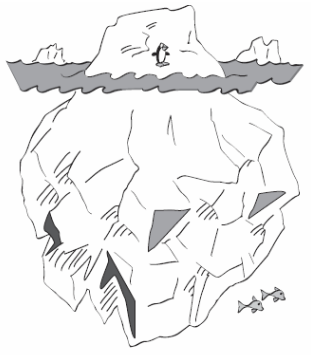
\includegraphics[width=\textwidth]{complexityHiding.png}
				\end{flushright}
			\end{column}
		\end{columns}
	\end{frame}

	\begin{frame}
		\frametitle{Изоляция возможных изменений}
		\begin{itemize}
			\item Определите элементы, изменение которых кажется вероятным
			\item Отделите элементы, изменение которых кажется вероятным
			\item Изолируйте элементы, изменение которых кажется вероятным
			\item Источники изменений
			\begin{itemize}
				\item Бизнес-правила
				\item Зависимости от оборудования
				\item Ввод-вывод
				\item Нестандартные возможности языка
				\item Сложные аспекты проектирования и конструирования
				\item Переменные статуса
				\item Размеры структур данных
				\item ...
			\end{itemize}
		\end{itemize}
	\end{frame}

	\begin{frame}
		\frametitle{Сопряжение и связность}
		\begin{itemize}
			\item \textbf{Сопряжение (Coupling)} --- мера того, насколько взаимозависимы разные модули в программе
			\item \textbf{Связность (Cohesion)} --- степень, в которой задачи, выполняемые одним модулем, связаны друг с другом
			\item Цель: слабое сопряжение и сильная связность
		\end{itemize}
	\end{frame}

	\section{Принципы SOLID}

	\begin{frame}
		\frametitle{Принципы SOLID}
		\begin{itemize}
			\item Single responsibility principle
			\item Open/closed principle
			\item Liskov substitution principle
			\item Interface segregation principle
			\item Dependency inversion principle
		\end{itemize}
	\end{frame}

	\begin{frame}
		\frametitle{Single responsibility principle}
		\begin{itemize}
			\item Каждый объект должен иметь одну обязанность
			\item Эта обязанность должна быть полностью инкапсулирована в класс
		\end{itemize}
		\begin{flushright}
			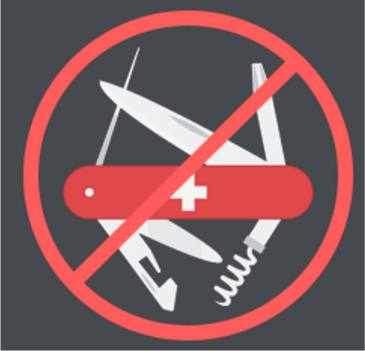
\includegraphics[width=0.25\textwidth]{singleResponsibility.png}
		\end{flushright}
	\end{frame}

	\begin{frame}
		\frametitle{Open/closed principle}
		\begin{itemize}
			\item программные сущности (классы, модули, функции и т. п.) должны быть открыты для расширения, но закрыты для изменения
			\begin{itemize}
				\item переиспользование через наследование
				\item неизменные интерфейсы
			\end{itemize}
		\end{itemize}
		\begin{flushright}
			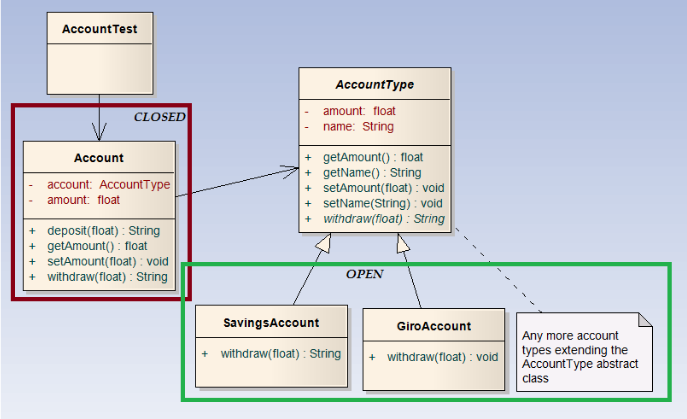
\includegraphics[width=0.5\textwidth]{openClosedPrinciple.png}
		\end{flushright}
	\end{frame}

	\begin{frame}
		\frametitle{Liskov substitution principle}
		\begin{itemize}
			\item Функции, которые используют базовый тип, должны иметь возможность использовать подтипы базового типа, не зная об этом
		\end{itemize}
		\begin{flushright}
			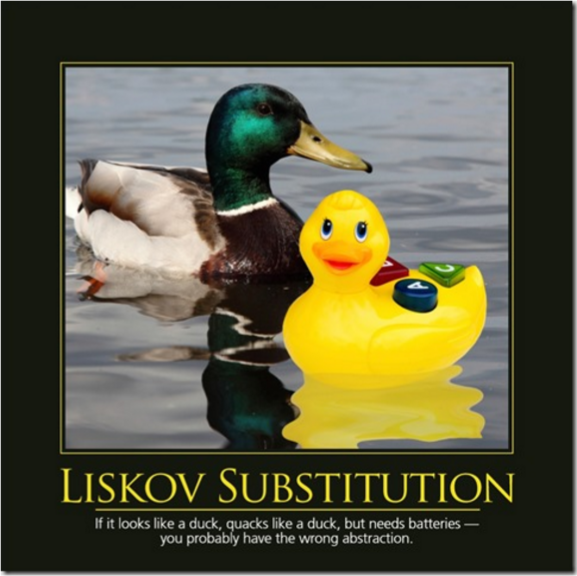
\includegraphics[width=0.4\textwidth]{liskovSubstitutionPrinciple.png}
		\end{flushright}
	\end{frame}

	\begin{frame}
		\frametitle{Interface segregation principle}
		\begin{itemize}
			\item Клиенты не должны зависеть от методов, которые они не используют
			\begin{itemize}
				\item слишком ``толстые'' интерфейсы необходимо разделять на более мелкие и специфические
			\end{itemize}
		\end{itemize}
		\begin{flushright}
			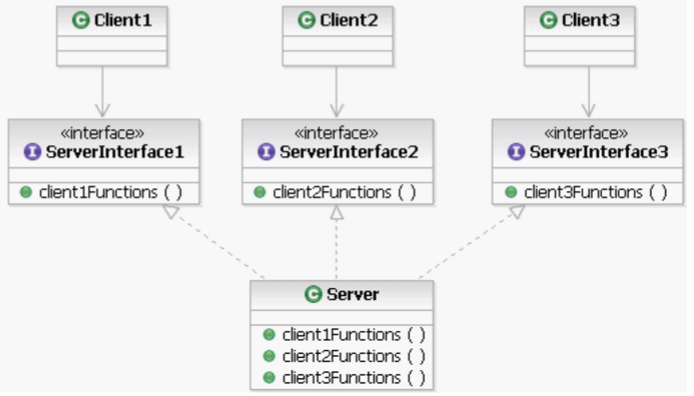
\includegraphics[width=0.5\textwidth]{interfaceSegregationPrinciple.png}
		\end{flushright}
	\end{frame}

	\begin{frame}
		\frametitle{Dependency inversion principle}
		\begin{itemize}
			\item Модули верхних уровней не должны зависеть от модулей нижних уровней. Оба типа модулей должны зависеть от абстракций
			\item Абстракции не должны зависеть от деталей. Детали должны зависеть от абстракций
		\end{itemize}
		\begin{flushright}
			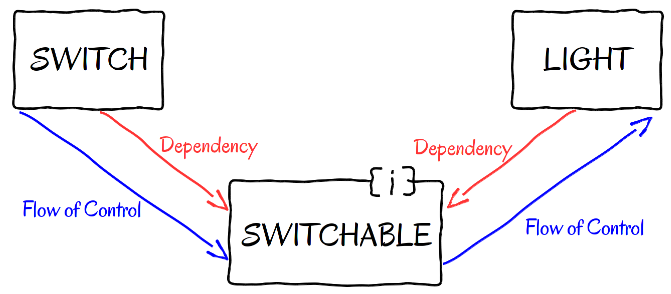
\includegraphics[width=0.5\textwidth]{dependencyInversionPrinciple.png}
		\end{flushright}
	\end{frame}

	\begin{frame}
		\frametitle{Закон Деметры}
		\begin{itemize}
			\item ``Не разговаривай с незнакомцами!''
			\item Объект A не должен иметь возможность получить непосредственный доступ к объекту C, если у объекта A есть доступ к объекту B, и у объекта B есть доступ к объекту C
			\begin{itemize}
				\item \mintinline{java}|book.pages.last.text|
				\item \mintinline{java}|book.pages().last().text()|
				\item \mintinline{java}|book.lastPageText()|
			\end{itemize}
		\end{itemize}
	\end{frame}

\end{document}